\section{Methodology}

\subsection{Overview}

Building on the observation that static analysis fails on 67--84\% of EvalPlus semantic
failures, we design a specification-aligned repair oracle that provides the structured
information necessary for targeted algorithmic repair. The design follows directly from
the insight that three orthogonal components are needed: intent anchoring (docstring),
behavioral gap specification (I/O counterexample), and deviation detection (actual
incorrect output). We call this the \textit{specification triple}.

The methodology has two phases: (1) an existence verification phase that establishes
the data infrastructure for reproducible repair experiments, and (2) a pre-registered
mechanism comparison phase that tests whether the triple outperforms blind reprompting.
This paper reports the existence phase; the mechanism phase is pre-registered and
awaits execution.

\subsection{The Specification Triple (Condition C)}

\textbf{Rationale.} The triple design is motivated by three converging mechanisms, each
supported by independent literature:

\begin{enumerate}
\item \textit{Docstring re-anchoring} (Step 1): Including the problem docstring's formal intent
   prevents the model from regenerating the same incorrect solution by re-anchoring
   it on the intended algorithm. \citet{Haeri2026} identify spec grounding as
   the primary driver of $+$38pp improvement; FeedbackEval \citep{Dai2025} shows
   severe degradation when docstrings are removed.

\item \textit{I/O counterexample} (Step 2): The failing test's input/expected-output pair
   provides a concrete behavioral gap --- a counterexample that specifies
   exactly where the model's behavior diverges from the specification.
   ContrastRepair \citep{Kong2024} demonstrates that contrastive I/O pairs
   outperform single failure messages (143/337 vs. 124 bugs).

\item \textit{Deviation detection} (Step 3): The model's actual incorrect output enables it to
   compare its behavior to the expected output and identify the specific algorithmic
   error. \citet{Iscan2026} confirms that content --- including actual output --- drives repair
   improvement (code$+$facts $+$18pp, p$=$0.00042), not mere re-exposure.
\end{enumerate}

\textbf{Prompt construction (Condition C):}

\begin{verbatim}
[Original problem prompt]

--- Specification Context ---
DOCSTRING (formal intent): [problem docstring]

FAILING TEST:
  Input: [plus_input[0] from EvalPlus]
  Expected output: [plus_output[0] from EvalPlus]

ACTUAL MODEL OUTPUT:
  [stored incorrect solution from solutions_cache.jsonl]
--- End Specification Context ---

Please repair the solution so that it passes all test cases.
\end{verbatim}

\begin{figure}[t]
\centering
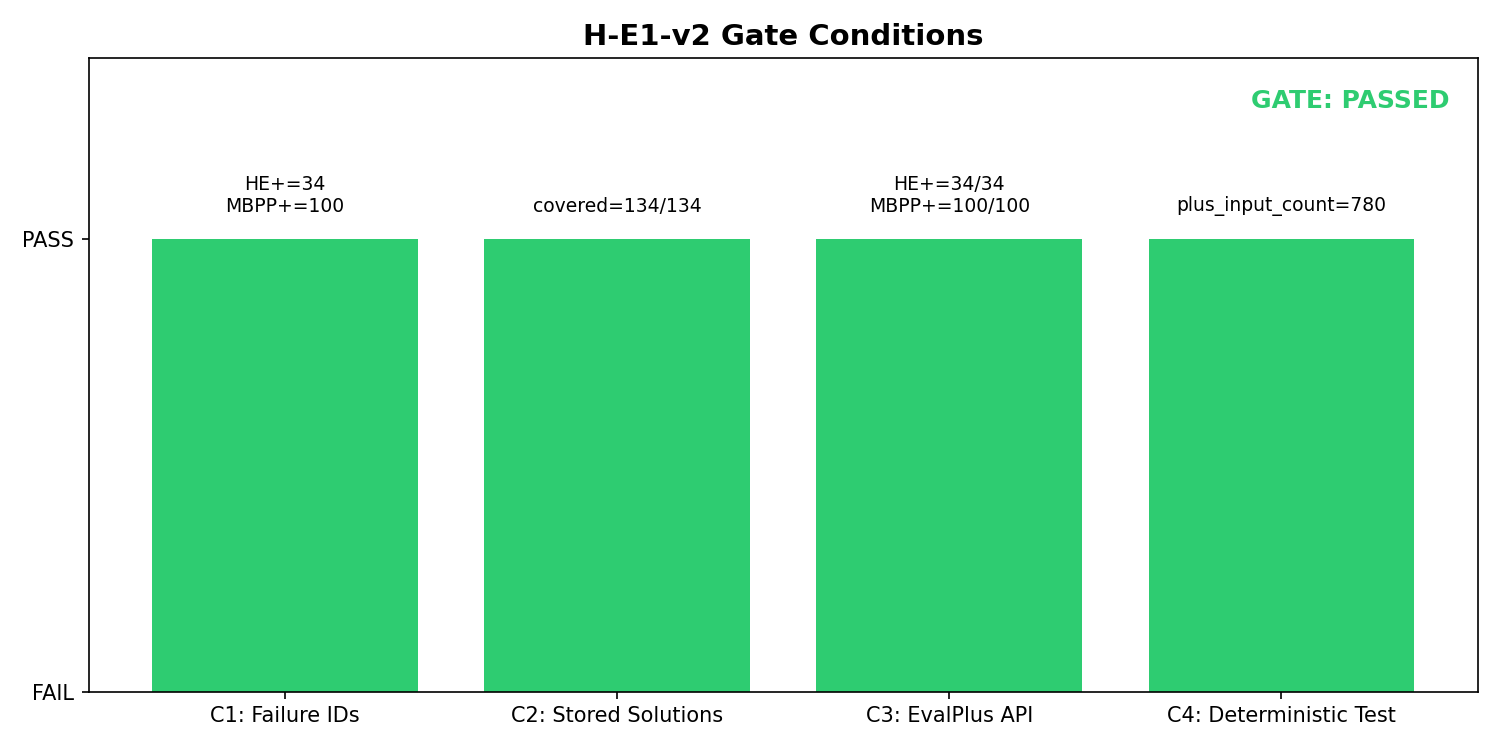
\includegraphics[width=0.8\textwidth]{figures/gate_conditions.png}
\caption{Verification of the four data infrastructure conditions (C1--C4) for the h-e1-v2 existence gate. All four conditions pass: failure IDs confirmed (C1), stored solutions verified (C2), EvalPlus API accessible (C3), deterministic test selection confirmed (C4).}
\label{fig:gate-conditions}
\end{figure}

\subsection{Experimental Conditions}

\begin{table}[h]
\centering
\caption{Summary of experimental conditions.}
\label{tab:conditions}
\begin{tabular}{lll}
\toprule
Condition & Description & API Calls \\
\midrule
A (Baseline) & Round-0 GPT-4o-mini output (existing h-e1 data) & 0 \\
B (Blind reprompt) & Original prompt + ``Please try again'' & 128 \\
C (Spec-aligned repair) & Original prompt + specification triple & 128 \\
\bottomrule
\end{tabular}
\end{table}

\textbf{Condition B} prompt: \texttt{[problem prompt]\textbackslash n\textbackslash nThe above solution is incorrect. Please try again.}

\subsection{Data Infrastructure}

\textbf{Source.} The 134-problem failure set is drawn from the h-e1 Run 2 archive.
We verify four conditions before any repair API calls (Figure~\ref{fig:gate-conditions}):

\begin{itemize}
\item \textbf{C1}: 134 failure IDs confirmed (34 HE$+$ $+$ 100 MBPP$+$)
\item \textbf{C2}: 134/134 stored GPT-4o-mini solutions in \texttt{solutions\_cache.jsonl}
\item \textbf{C3}: All 134 IDs accessible via EvalPlus API
\item \textbf{C4}: Deterministic test selection via \texttt{plus\_input[0]} confirmed (780 test cases for sample task)
\end{itemize}

Six tasks with empty \texttt{plus\_fail\_tests} yield a 128-task working set.

\subsection{Statistical Design}

\textbf{Primary (P1, h-m1).} One-tailed McNemar's test on Condition B vs. C fix outcomes
across 128 problems. Success: p $<$ 0.05 (direction: C $>$ B). Yates' correction if any
cell $<$ 5; Fisher's exact fallback if discordant pairs $<$ 25.

\textbf{Secondary (P2, h-m2).} One-tailed McNemar for C vs. A; fix rate threshold $\geq$ 15\%.

\textbf{Exploratory (P3, h-c1).} Stratified fix rates by benchmark type (34 HE$+$ vs. 100
MBPP$+$) with Fisher's exact test; directional comparison only.

\textbf{Model.} GPT-4o-mini, temperature$=$0.2, seed$=$42 (pre-registered).
